\documentclass[aspectratio=169]{beamer}
\usetheme{Boadilla}
\usecolortheme{seahorse}
\usepackage[T1]{fontenc}
\usepackage{lmodern}
\usepackage{booktabs}
\usepackage{amsmath}
\usepackage{xcolor}
\usepackage{tikz}
\usetikzlibrary{arrows.meta,positioning,fit,backgrounds}

\setbeamertemplate{navigation symbols}{}
\setbeamertemplate{itemize items}[circle]

\newcommand{\keybox}[1]{%
  \begin{center}
  \colorbox{black!8}{\parbox{0.92\textwidth}{\centering #1}}
  \end{center}}

\newcommand{\meas}{{\color{blue!55!black}\textbf{measured}}}
\newcommand{\proj}{{\color{orange!75!black}\textbf{projected}}}

\title{A Frontier Model That Behaves Itself}
\subtitle{colibr\`i on LIBR compute --- what it is, how you use it, and how fast it really goes}
\author{\texttt{libr-local-llm} --- the next phase}
\date{}

\begin{document}

\frame{\titlepage}

%----------------------------------------------------------
\begin{frame}{The whole thing in one sentence}

\keybox{\large A \textbf{744-billion-parameter} model, running on one LIBR node, that reads PHI,
answers one hard question at a time, and hands the node back when somebody else needs it.}

\vspace{0.7em}
\begin{columns}[T]
\begin{column}{0.47\textwidth}
{\small\textbf{What you gain}
\begin{itemize}\small
\item Frontier-scale weights, entirely on-premises
\item Reasoning quality no 30B model reaches
\item Tool calling, so a real terminal client works
\item An API key --- the first engine here that has one
\end{itemize}}
\end{column}
\begin{column}{0.47\textwidth}
{\small\textbf{What it costs}
\begin{itemize}\small
\item \textbf{6--12 tokens per second}
\item \textbf{27 minutes} to start from cold
\item One generation at a time, ever
\item About one whole node of the six
\end{itemize}}
\end{column}
\end{columns}

\vspace{0.6em}
\keybox{\textbf{Read those two columns together.} This is a \textbf{consultant}, not an agent loop.
One hard question and 80 seconds is a good trade. Forty tool calls is not, and no engineering in
this deck changes that.}

\end{frame}

%----------------------------------------------------------
\begin{frame}{Why a 744B model runs on a machine that cannot hold it}

A 744B mixture-of-experts activates only about \textbf{40B parameters per token} --- and only the
\emph{routed experts} change from one token to the next.

\begin{center}
\resizebox{0.95\textwidth}{!}{%
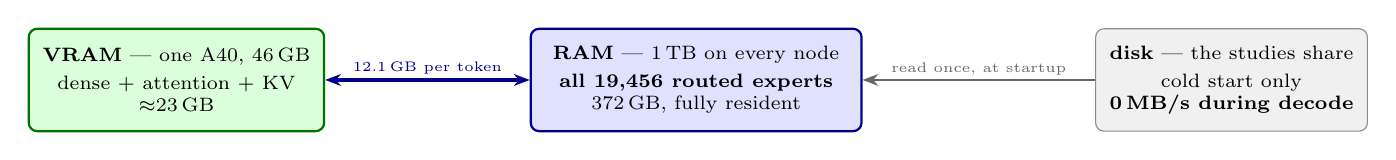
\begin{tikzpicture}[
  font=\scriptsize,
  >={Stealth[length=2mm]},
  tier/.style={rounded corners=3pt, align=center, inner sep=5pt, minimum height=13mm},
  lbl/.style={font=\tiny, inner sep=1.5pt}
]
\node[tier, draw=green!45!black, thick, fill=green!14, minimum width=32mm] (v) at (0,0)
  {\textbf{VRAM} --- one A40, 46\,GB\\[2pt]dense + attention + KV\\$\approx$23\,GB};
\node[tier, draw=blue!55!black, thick, fill=blue!12, minimum width=42mm] (r) at (6.6,0)
  {\textbf{RAM} --- 1\,TB on every node\\[2pt]\textbf{all 19,456 routed experts}\\372\,GB, fully resident};
\node[tier, draw=black!45, fill=black!6, minimum width=32mm] (d) at (13.4,0)
  {\textbf{disk} --- the studies share\\[2pt]cold start only\\\textbf{0\,MB/s during decode}};
\draw[->, thick, black!60] (d) -- node[lbl, above] {read once, at startup} (r);
\draw[<->, very thick, blue!55!black] (r) -- node[lbl, above] {12.1\,GB per token} (v);
\end{tikzpicture}}
\end{center}

\vspace{0.3em}
\textbf{Think of it as a JIT, but for weights.} A compiler JIT never compiles the whole program --- it
watches what actually runs. colibr\`i makes the same bet: parameters are not state to be held, they
are \textbf{data to be staged}, exactly when the router proves they are needed.

\vspace{0.5em}
\keybox{\textbf{Placement decides speed and nothing else.} The router's decisions and the weights'
precision are identical whether an expert answered from VRAM or from disk. You cannot make it
\emph{wrong} by placing it badly --- only slow.}

\end{frame}

%----------------------------------------------------------
\begin{frame}{Where the speed comes from, and where it stops}

Every token has to read the experts it routes to. That single fact is the whole ceiling.

\keybox{\parbox{0.85\textwidth}{\centering\vspace{0.2em}
\texttt{8 experts $\times$ 20.1\,MB $\times$ 75 layers = \textbf{12.1\,GB touched per token}}

\vspace{0.4em}
\texttt{tokens/second = memory bandwidth $\div$ 12.1\,GB}
\vspace{0.2em}}}

\vspace{0.7em}
On the reference machine colibr\`i was tuned on, the expert path sustained \meas\ \textbf{19.7 GB/s}
--- only 23\% of that host's memory --- and the ceiling was \textbf{3.0 tok/s}. Everything else in
the engine is bounded above by that line.

\vspace{0.6em}
\begin{center}
\small
\begin{tabular}{@{}lrr@{}}
\toprule
& \textbf{bandwidth} & \textbf{ceiling} \\
\midrule
reference host, as measured & 19.7 GB/s & 3.0 tok/s \\
reference host, memory saturated & 85 GB/s & 13.0 tok/s \\
\textbf{our node} (2$\times$ Ice Lake, 8 channels/socket) & \textbf{$\sim$410 GB/s theoretical} & --- \\
\bottomrule
\end{tabular}
\end{center}

\vspace{0.5em}
{\scriptsize The gap between the first two rows is why this is a \emph{tuning} problem rather than a
hardware problem, and the third row is why our node is worth tuning.}

\end{frame}

%----------------------------------------------------------
\begin{frame}{Our node is the good case, for two reasons}

\begin{center}
\scriptsize
\renewcommand{\arraystretch}{1.15}
\begin{tabular}{@{}p{0.16\textwidth}p{0.37\textwidth}p{0.40\textwidth}@{}}
\toprule
& \textbf{reference host (4$\times$A6000)} & \textbf{LIBR compute30\emph{x}} \\
\midrule
CPU & EPYC Zen 2, 24c/48t, \textbf{AVX2 only} & 2$\times$ Xeon Ice Lake, \textbf{48c/96t, AVX-512 + VNNI} \\
RAM & 264\,GB DDR4-2400, $\sim$85\,GB/s & \textbf{1\,TB} DDR4-3200, $\sim$410\,GB/s \\
residency & 367 of 429\,GB --- \textbf{disk stays in the path} & \textbf{372 of 1024\,GB --- disk leaves entirely} \\
GPU & 4$\times$ A6000 48\,GB, sm\_86 & 1--4$\times$ A40 46\,GB, \textbf{same generation} \\
storage & local NVMe, 2.9\,GB/s & NFS, 0.23\,GB/s --- 12$\times$ worse, \textbf{cold start only} \\
\bottomrule
\end{tabular}
\end{center}

\vspace{0.7em}
Two rows matter and the rest is detail.

\begin{itemize}\small
\item \textbf{AVX-512 VNNI} gives the int4 kernels a path the reference host did not have. colibr\`i
      picks it automatically --- \emph{if you compile for this machine}. The default build target is
      AVX2 and would throw it away.
\item \textbf{1\,TB of RAM} holds the entire model. That removes disk from decode permanently, which
      is the configuration behind every good number colibr\`i has ever published, and which the
      reference host could not reach.
\end{itemize}

\end{frame}

%----------------------------------------------------------
\begin{frame}{The counter-intuitive result: one GPU, not four}

Having 1\,TB of RAM changes what the GPU is \emph{for}.

\begin{center}
\small
\begin{tabular}{@{}p{0.44\textwidth}p{0.50\textwidth}@{}}
\toprule
\textbf{What the GPU is for} & \textbf{What more GPUs would add} \\
\midrule
The \textbf{dense and attention} tensors.
$\approx$12\,GB, plus $\approx$11\,GB of KV cache.
\textbf{23\,GB --- one A40 holds it.} &
More \emph{experts} resident in VRAM instead of RAM.
Which, once the model is RAM-resident, is worth\ldots \\
\midrule
\meas\ \textbf{$\times$2.8} (1.53 $\rightarrow$ 4.26 tok/s) &
\meas\ \textbf{under 2\%} \\
\bottomrule
\end{tabular}
\end{center}

\vspace{0.4em}
{\small colibr\`i's own controlled A/B: VRAM-heavy (188\,GB) and balanced (176\,GB) measured
\textbf{2.81 vs 2.78 tok/s} --- indistinguishable. Raising the \emph{RAM} budget by 30\,GB bought
\textbf{+25\%}.}

\vspace{0.4em}
\keybox{\textbf{So the service never needs compute306.} It takes one A40 of the seven on the cluster
and leaves the only four-GPU node completely alone. That is the strongest citizenship position
available to us, and it falls out of the arithmetic rather than out of good manners.}

\end{frame}

%----------------------------------------------------------
\begin{frame}{The number, and where it comes from}

colibr\`i's source carries measurements taken on a \textbf{2-socket Ice Lake, 48 cores, model fully
resident} --- the same CPU generation, core count, and residency condition as ours.

\begin{center}
\scriptsize
\begin{tabular}{@{}lrrl@{}}
\toprule
\textbf{Condition} & \textbf{tok/s} & \textbf{expert-matmul} & \textbf{source} \\
\midrule
before the VNNI int4 kernel & 3.65 & 67.8 GB/s & \texttt{colibri.c:541} \\
\textbf{with AVX-512 VNNI} (automatic, if compiled for it) & \textbf{3.85} & \textbf{89.5 GB/s} & \texttt{colibri.c:541} \\
baseline of the next campaign & 4.20 & --- & \texttt{colibri.c:554} \\
\textbf{plus \texttt{XEXP=1}} (one thread team per block) & \textbf{4.68} & \textbf{131.9 GB/s} & \texttt{colibri.c:554} \\
\bottomrule
\end{tabular}
\end{center}

\vspace{0.4em}
{\small Those runs are \textbf{CPU-side} --- none used the GPU for the dense path. Add that
$\times$2.8 lever, partially, and you get:}

\keybox{\proj\ \textbf{6--12 tok/s, most likely around 8.} A projection built from measured parts:
a measured 4.68 tok/s floor on our CPU class, times a partial capture of a measured GPU lever. The
first real run on our hardware replaces this line.}

\vspace{0.2em}
{\scriptsize \texttt{XEXP=1} was \textbf{neutral or negative on a 24-core box}, which is why it is
opt-in. On 48 cores it is the largest CPU-side lever there is.}

\end{frame}

%----------------------------------------------------------
\begin{frame}{Four things that do not help, with evidence}

\begin{center}
\scriptsize
\renewcommand{\arraystretch}{1.1}
\begin{tabular}{@{}p{0.28\textwidth}p{0.64\textwidth}@{}}
\toprule
\textbf{The obvious idea} & \textbf{What was measured} \\
\midrule
More GPUs & Under 2\% once the model is RAM-resident. See the previous slide. \\[0.3em]
More users at once & The engine \emph{serialises}. 1.32 / 1.51 / 1.46 tok/s aggregate at 1 / 2 / 4
clients --- concurrency divides throughput, it does not scale it. \\[0.3em]
Disk prefetch machinery & Turning it \textbf{off} was worth \textbf{+26\%}. Once experts are
resident the disk reads 0\,MB/s, so prefetch only burns CPU --- the scarce resource. \\[0.3em]
Maximising memory & With the dense path on the CPU, a 176\,GB configuration measured \emph{slower}
than a 99\,GB one. Gains also do not compose. \\
\bottomrule
\end{tabular}
\end{center}

\vspace{0.5em}
\keybox{\small \textbf{And one hidden trap that invalidates naive benchmarking entirely.}
colibr\`i keeps a learned routing profile on disk that survives restarts. An \emph{identical}
configuration measured \textbf{5.46 tok/s and then 2.56} with no parameter changed. Every
measurement must snapshot and restore that file, or it measures nothing.}

\end{frame}

%----------------------------------------------------------
\begin{frame}{The real constraint is the 27-minute cold start}

{\small 372\,GB off the studies share at \meas\ 230\,MB/s. That number, not the GPU, drives every
remaining decision --- and it collides with how this cluster's partitions are configured.}

\begin{center}
\scriptsize
\renewcommand{\arraystretch}{1.1}
\begin{tabular}{@{}lccp{0.44\textwidth}@{}}
\toprule
\textbf{Partition} & \textbf{Time limit} & \textbf{Can be frozen?} & \textbf{Verdict} \\
\midrule
\texttt{c3\_short} & \textbf{9 h} & no & 27 min of every 9 h is a reload --- \textbf{5\% duty lost, 2.7 restarts a day} \\[0.3em]
\texttt{c3} & 7 d & \textbf{yes, silently} & a \texttt{c3\_short} job can \texttt{SIGSTOP} it; the client just hangs \\[0.3em]
\texttt{c3\_accel} & 7 d & no & the only long-\emph{and}-safe option --- but it is the four-GPU node we just proved we do not need \\
\bottomrule
\end{tabular}
\end{center}

\vspace{0.3em}
{\small \textbf{The inversion worth noticing.} Having argued we do not need compute306's
\emph{cards}, the strongest reason to run there is its \emph{partition} --- the only place offering
a 7-day life with no preemption exposure.}

\vspace{0.3em}
\keybox{\small \textbf{The plan says \texttt{c3\_short}, reluctantly}, and takes the 5\%. Holding
the only four-GPU node for a service that does not need four GPUs is indefensible. \textbf{One test
may settle it}: a node has 1\,TB of RAM and the model is 372\,GB, so a restart on the \emph{same}
node may find it still in page cache.}

\end{frame}

%----------------------------------------------------------
\begin{frame}{The system is four boxes}

\begin{center}
\resizebox{0.75\textwidth}{!}{%
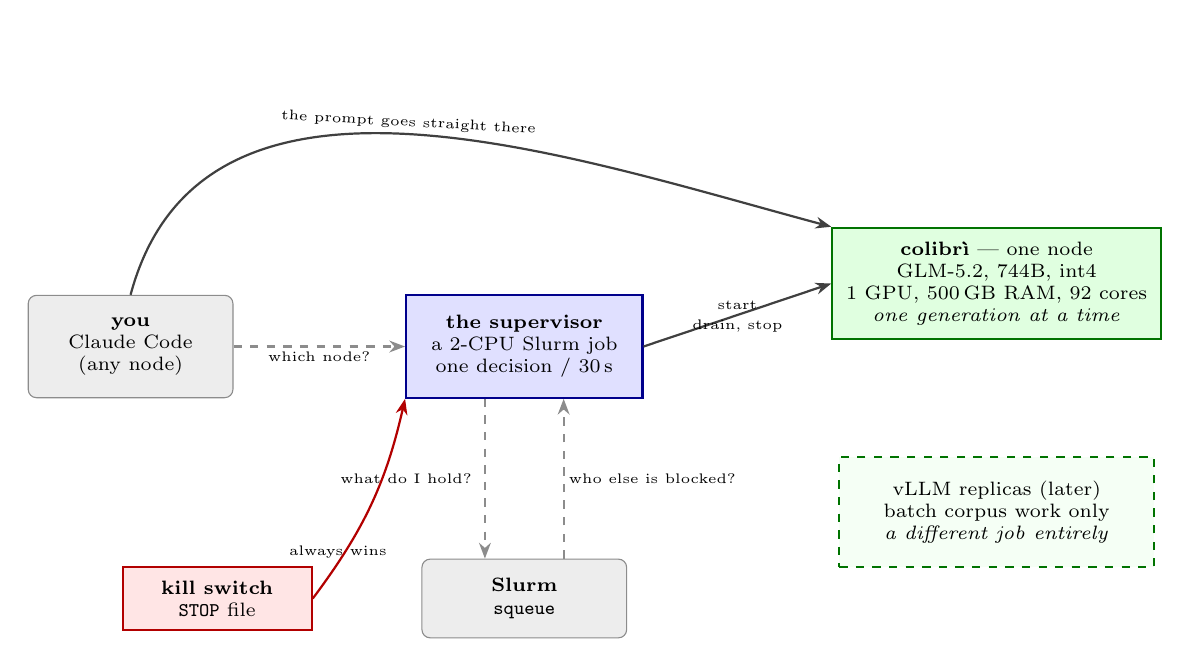
\begin{tikzpicture}[
  font=\scriptsize,
  >={Stealth[length=2mm]},
  box/.style={draw=black!45, rounded corners=3pt, fill=black!7,
              align=center, inner sep=4pt, minimum height=10mm, minimum width=26mm},
  ctrl/.style={draw=blue!55!black, thick, fill=blue!12,
               align=center, inner sep=4pt, minimum height=10mm, minimum width=30mm},
  gpu/.style={draw=green!45!black, thick, fill=green!12,
              align=center, inner sep=5pt, minimum height=14mm, minimum width=40mm},
  kill/.style={draw=red!70!black, thick, fill=red!10,
               align=center, inner sep=3pt, minimum height=8mm, minimum width=24mm},
  flow/.style={->, thick, draw=black!75},
  ask/.style={->, thick, draw=black!45, dashed},
  lbl/.style={font=\tiny, inner sep=1.5pt}
]
\node[box, minimum height=13mm]  (you)   at (0,0.8)    {\textbf{you}\\Claude Code\\(any node)};
\node[ctrl, minimum height=13mm] (sup)   at (5.0,0.8)  {\textbf{the supervisor}\\a 2-CPU Slurm job\\one decision / 30\,s};
\node[box]                       (slurm) at (5.0,-2.4) {\textbf{Slurm}\\\texttt{squeue}};
\node[kill]                      (stop)  at (1.1,-2.4) {\textbf{kill switch}\\\texttt{STOP} file};
\node[gpu] (b1) at (11.0,1.6) {\textbf{colibr\`i} --- one node\\GLM-5.2, 744B, int4\\1 GPU, 500\,GB RAM, 92 cores\\\emph{one generation at a time}};
\node[gpu, fill=green!4, dashed] (b2) at (11.0,-1.3) {vLLM replicas (later)\\batch corpus work only\\\emph{a different job entirely}};

\draw[ask] (you.east) -- node[lbl, below] {which node?} (sup.west);
\draw[ask] ([xshift=-5mm]sup.south) -- node[lbl, left, xshift=-1mm] {what do I hold?} ([xshift=-5mm]slurm.north);
\draw[ask] ([xshift=5mm]slurm.north) -- node[lbl, right] {who else is blocked?} ([xshift=5mm]sup.south);
\draw[flow] (sup.east) -- node[lbl, above] {start} node[lbl, below] {drain, stop} (b1.west);
\draw[flow, draw=red!70!black] (stop.east) to[bend right=12] node[lbl, above, pos=0.18] {always wins} (sup.south west);
\draw[flow] (you.north) to[out=75, in=165] node[lbl, above, sloped] {the prompt goes straight there} (b1.north west);
\end{tikzpicture}}
\end{center}

\vspace{-0.2em}
{\scriptsize \textbf{The supervisor remembers nothing.} Every 30 seconds it asks Slurm what it holds
and who is waiting, then takes \emph{one} action. It keeps no state, so a crash loses none --- and
the backend keeps serving while it is gone.}

\end{frame}

%----------------------------------------------------------
\begin{frame}{What you actually type --- and it is Claude Code}

{\small colibr\`i speaks the \textbf{Anthropic Messages API} on the same port as everything else,
and GLM-5.2 supports tool calling. So the client is the one you already use --- three environment
variables, no shim:}

\keybox{\parbox{0.7\textwidth}{\ttfamily\small
export ANTHROPIC\_BASE\_URL=http://127.0.0.1:8000 \\
export ANTHROPIC\_API\_KEY=\emph{your key} \\
export ANTHROPIC\_MODEL=glm-5.2-colibri \\
claude}}

\vspace{0.4em}
\begin{center}
\scriptsize
\begin{tabular}{@{}ll@{}}
\toprule
\textbf{Command} & \textbf{What happens} \\
\midrule
\texttt{fleet code} & sets those three, steps onto the backend's node, starts Claude Code \\
\texttt{fleet status} & what is up, what is warm, what it is waiting on \\
\texttt{fleet up} / \texttt{fleet down} & start the supervisor / stop everything and stay stopped \\
\bottomrule
\end{tabular}
\end{center}

\vspace{0.4em}
\keybox{\small \textbf{And colibr\`i has an API key, which ollama never did.} \texttt{COLI\_API\_KEY} closes
a gap this repo has had recorded as \emph{live} since August: a loopback port is not a boundary
against other users on the same node, and until now nothing else was one either.}

\end{frame}

%----------------------------------------------------------
\begin{frame}{Restarting itself, and the switch that stops it}

\begin{center}
\resizebox{0.78\textwidth}{!}{%
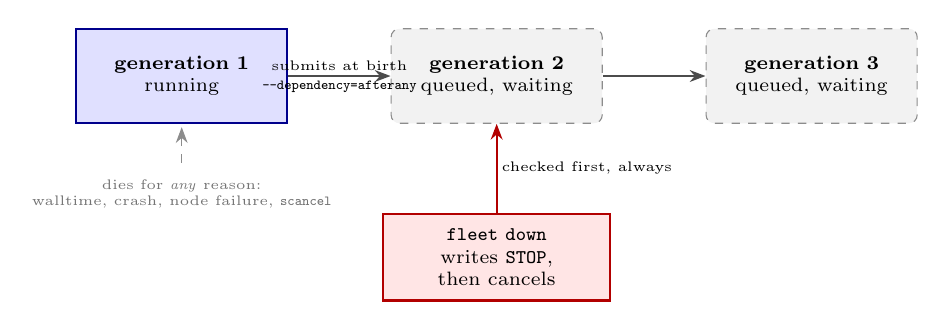
\begin{tikzpicture}[
  font=\scriptsize,
  >={Stealth[length=2mm]},
  gen/.style={draw=blue!55!black, thick, fill=blue!12,
              align=center, inner sep=4pt, text width=24mm, minimum height=12mm},
  pend/.style={draw=black!45, dashed, rounded corners=3pt, fill=black!5,
               align=center, inner sep=4pt, text width=24mm, minimum height=12mm},
  kill/.style={draw=red!70!black, thick, fill=red!10,
               align=center, inner sep=4pt, text width=26mm, minimum height=11mm},
  flow/.style={->, thick, draw=black!70},
  lbl/.style={font=\tiny, inner sep=1.5pt}
]
\node[gen]  (g1) at (0,0)    {\textbf{generation 1}\\running};
\node[pend] (g2) at (4.0,0)  {\textbf{generation 2}\\queued, waiting};
\node[pend] (g3) at (8.0,0)  {\textbf{generation 3}\\queued, waiting};
\node[kill] (k)  at (4.0,-2.3) {\textbf{\texttt{fleet down}}\\writes \texttt{STOP}, then cancels};
\draw[flow] (g1) -- node[lbl, above] {submits at birth}
                   node[lbl, below] {\texttt{-{}-dependency=afterany}} (g2);
\draw[flow] (g2) -- (g3);
\draw[flow, draw=red!70!black] (k) -- node[lbl, right] {checked first, always} (g2);
\node[lbl, text=black!55, align=center] at (0,-1.5) {dies for \emph{any} reason:\\walltime, crash,
node failure, \texttt{scancel}};
\draw[->, black!45, dashed] (0,-1.1) -- (0,-0.65);
\end{tikzpicture}}
\end{center}

\vspace{0.2em}
{\small \textbf{Each generation submits its successor the moment it starts}, with a dependency that
fires on \emph{any} termination. A pending job costs nothing, so the queued successor is free
insurance.}

\vspace{0.3em}
\keybox{\small \textbf{The kill switch is a file, not a signal.} \texttt{fleet down} writes
\texttt{STOP} \emph{before} it cancels anything, so the successor starts, reads it, and exits in two
seconds. It works when the supervisor is wedged and when its node is gone --- a kill switch that
depends on the thing it kills is not one.}

\end{frame}

%----------------------------------------------------------
\begin{frame}{Citizenship --- and where the pivot costs something}

\begin{center}
\resizebox{0.92\textwidth}{!}{%
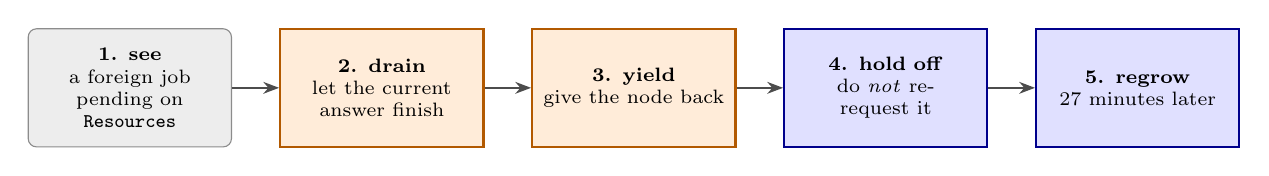
\begin{tikzpicture}[
  font=\scriptsize,
  >={Stealth[length=2mm]},
  stg/.style={draw=black!45, rounded corners=3pt, fill=black!7,
              align=center, inner sep=4pt, text width=23mm, minimum height=15mm},
  hot/.style={draw=orange!70!black, thick, fill=orange!15,
              align=center, inner sep=4pt, text width=23mm, minimum height=15mm},
  cool/.style={draw=blue!55!black, thick, fill=blue!12,
               align=center, inner sep=4pt, text width=23mm, minimum height=15mm},
  flow/.style={->, thick, draw=black!70}
]
\node[stg]  (s1) at (0,0)    {\textbf{1. see}\\a foreign job pending on \texttt{Resources}};
\node[hot]  (s2) at (3.2,0)  {\textbf{2. drain}\\let the current answer finish};
\node[hot]  (s3) at (6.4,0)  {\textbf{3. yield}\\give the node back};
\node[cool] (s4) at (9.6,0)  {\textbf{4. hold off}\\do \emph{not} re-request it};
\node[cool] (s5) at (12.8,0) {\textbf{5. regrow}\\27 minutes later};
\draw[flow] (s1) -- (s2); \draw[flow] (s2) -- (s3);
\draw[flow] (s3) -- (s4); \draw[flow] (s4) -- (s5);
\end{tikzpicture}}
\end{center}

\vspace{0.5em}
\begin{columns}[T]
\begin{column}{0.47\textwidth}
{\small\textbf{What survives, and it is real}
\begin{itemize}\small
\item We hold \textbf{one GPU of seven}, never compute306
\item One backend. Never two. Ever.
\item Idle release still fires --- on a 3-hour clock, not 30 minutes
\end{itemize}}
\end{column}
\begin{column}{0.47\textwidth}
{\small\textbf{What it honestly costs}
\begin{itemize}\small
\item A yield takes the service down for \textbf{27 minutes}
\item $\sim$92 CPUs and 500\,GB billed continuously
\item So it will yield \emph{reluctantly}, and rarely
\end{itemize}}
\end{column}
\end{columns}

\vspace{0.5em}
{\scriptsize A 27-minute asset released over a lunch break is thrashing, and a fleet that thrashes is
worse than a fleet that is simply smaller. If the standing cost is unacceptable, the answer is a
shorter walltime --- not a cleverer policy.}

\end{frame}

%----------------------------------------------------------
\begin{frame}{vLLM is the other half, and not a competitor}

colibr\`i serves \textbf{one generation at a time}, at any tuning, forever. So it cannot do corpus
work --- and the two engines stop overlapping entirely.

\begin{center}
\small
\begin{tabular}{@{}p{0.14\textwidth}p{0.38\textwidth}p{0.40\textwidth}@{}}
\toprule
& \textbf{colibr\`i} & \textbf{vLLM} \\
\midrule
workload & one hard question, interactively & ten thousand documents, unattended \\
model & GLM-5.2 744B int4 & MedGemma 27B, 8-bit \\
shape & one long-lived backend, single slot & N single-GPU replicas, batched \\
plane & HTTP on loopback & \textbf{filesystem queue --- no socket at all} \\
for & frontier reasoning on PHI & PSYCH-ASR Stage 3c, schema-guided JSON \\
\bottomrule
\end{tabular}
\end{center}

\vspace{0.5em}
\keybox{\small \textbf{Do not build a router between these two.} They share no caller and no workload. The
arbitration layer the original design was going to need has been deleted, which is the pivot's one
unambiguous simplification.}

\vspace{0.4em}
{\scriptsize The batch queue is also the strongest PHI control in the design, because it removes
the socket entirely: a worker killed mid-item costs one item, not the pass.}

\end{frame}

%----------------------------------------------------------
\begin{frame}{Which model, inside colibr\`i}

{\small Eight families run on the same engine. The filter is brutal: it must fit in 1\,TB of RAM,
\textbf{and} support tool calling, or a terminal client cannot drive it.}

\begin{center}
\scriptsize
\renewcommand{\arraystretch}{1.15}
\begin{tabular}{@{}lrrcp{0.34\textwidth}@{}}
\toprule
\textbf{Model} & \textbf{total / active} & \textbf{container} & \textbf{tools} & \textbf{verdict} \\
\midrule
\textbf{GLM-5.2} & 744B / 40B & \textbf{372 GB} & \textbf{yes} & \textbf{the default} --- every number in this deck belongs to it \\
DeepSeek V4 Flash & 284B / \textbf{13B} & 167 GB & \textbf{yes} & \textbf{measure it.} One third the active parameters could mean real speed \\
GLM-5.3-Flash & 321B / 40B & 195 GB & yes & a lighter GLM; needs conversion \\
Inkling & 975B / 41B & 469 GB & \textbf{no} & unusable --- rejects tool calls with HTTP 400 \\
Kimi K3 & 2.8T / 104B & \textbf{1.6 TB} & yes & \textbf{does not fit in RAM.} Dead here \\
\bottomrule
\end{tabular}
\end{center}

\vspace{0.5em}
\keybox{\small \textbf{Quality is not free, and the number is known.} GLM-5.2's int4 container measures
\textbf{$-$8.2 percentage points} against the unquantized model, concentrated on the hardest
questions. Whether 744B at int4 beats a well-served smaller model at 8-bit \emph{for our tasks} is a
blind side-by-side nobody has run. The pivot makes that comparison more important, not less.}

\end{frame}

%----------------------------------------------------------
\begin{frame}{Build order --- and you can stop early}

\begin{center}
\scriptsize
\renewcommand{\arraystretch}{1.15}
\begin{tabular}{@{}llp{0.46\textwidth}@{}}
\toprule
\textbf{Phase} & \textbf{What lands} & \textbf{Exit criterion} \\
\midrule
P0 & ten verification tests & \textbf{a real tok/s number on our hardware}, under the snapshot protocol \\
P1 & one backend, tuned, run by hand & Claude Code finishes a real task against it, with a tool call \\
P2 & the sbatch, \texttt{fleet up} / \texttt{status} / \texttt{down} & one command, and it refuses to claim success before a token exists \\
P3 & supervisor, chain, kill switch & survives two rollovers; \texttt{fleet down} makes it stay down \\
P4 & idle release, caps, yield, hold-off & yields to a real blocked job, does not take the node back early \\
P5 & vLLM + the batch queue & a corpus pass survives a worker being killed \\
\bottomrule
\end{tabular}
\end{center}

\vspace{0.5em}
\keybox{\small \textbf{Stop after P1 and you already have what was asked for}, run by hand. P2--P4 are what
make it survive being left alone. \textbf{P0 comes first and is not optional} --- the previous plan
could build its control plane first because ollama was already proven. Nothing here is.}

\end{frame}

%----------------------------------------------------------
\begin{frame}{Five decisions that are yours, not mine}

\begin{center}
\scriptsize
\renewcommand{\arraystretch}{1.2}
\begin{tabular}{@{}p{0.46\textwidth}p{0.24\textwidth}p{0.22\textwidth}@{}}
\toprule
\textbf{Question} & \textbf{Proposed} & \textbf{Cost if changed} \\
\midrule
Partition: 9-hour and safe, or 7-day on the four-GPU node? & \texttt{c3\_short}, reluctantly & 5\% duty lost, versus holding the scarcest node \\
Is $\sim$92 CPUs and 500\,GB on one of six nodes, continuously, acceptable? & \textbf{it has to be} & if not, the service does not exist in this form \\
GLM-5.2 only, or measure DeepSeek V4 Flash first? & measure both & 13B active vs 40B is a large potential speed difference \\
Claude Code or opencode as the client? & \textbf{Claude Code} & colibr\`i speaks Anthropic natively; opencode stays as fallback \\
\textbf{Is 6--12 tok/s acceptable for the work you have in mind?} & \textbf{as a consultant, yes} & as an agent loop, \textbf{no}, and nothing here changes that \\
\bottomrule
\end{tabular}
\end{center}

\vspace{0.5em}
{\scriptsize Recorded as open in \texttt{FLEET-BUILD.md} §13. Answer them once, with a date, and the
implementation stops guessing.}

\end{frame}

%----------------------------------------------------------
\begin{frame}{What ``done'' looks like}

\keybox{\parbox{0.9\textwidth}{\vspace{0.3em}
You type \texttt{fleet code} and Claude Code opens against a \textbf{744-billion-parameter model
running on LIBR hardware}, which may read PHI, because nothing leaves the building.

You ask it one hard question. It thinks for eighty seconds and answers well.

Overnight the fleet releases the node. In the morning you pay 27 minutes, once, and carry on.

If a colleague's GPU job goes pending, the fleet finishes your answer and gives the node back ---
and the log says so, with their job id, when anybody asks.
\vspace{0.3em}}}

\vspace{0.8em}
Nothing in that paragraph needs an administrator, a login-node daemon, or a person watching.

\vspace{0.7em}
\begin{center}
\textbf{It is frontier-scale.} \quad \textbf{It is on-premises.} \quad \textbf{It is eight tokens a
second.}
\end{center}

\vspace{0.3em}
\begin{center}
{\small Two of those three are the reason to build it. The third is why it is a consultant.}
\end{center}

\end{frame}

\end{document}
